% This document must be compiled with LuaLaTeX
\documentclass[12pt,article]{memoir}

\usepackage[letterpaper, portrait, margin=1in]{geometry}	% Standard page setup
\usepackage[USenglish]{babel}								% English typsetting conventions
\usepackage{fancyhdr}										% Headers and footers
\usepackage{graphicx}										% Additional graphics options
\usepackage{xcolor}											% Better colors
\usepackage{xpatch}											% Better macro patches
\usepackage{hyperref}										% Hyperlinks
\usepackage{fontspec}										% Custom fonts
\usepackage{tikz}											% Graphics creation
\usepackage{float}											% Figure positioning
\usepackage{tabu}											% Better tables
\usepackage[style=ieee, backend=biber]{biblatex}			% Bibliography
\usepackage[font={small,it}]{caption}						% Italic captions
\setsansfont{NeueHaasUnicaPro}
\usetikzlibrary{calc}
\usepackage[yyyymmdd]{datetime} % change date format to yyyy/mm/dd to fit ISO8601

\renewcommand{\familydefault}{\sfdefault} % set font
\renewcommand{\dateseparator}{--} % change date-seperators to - to fit ISO8601

\renewcommand\contentsname{Table of Contents}

\chapterstyle{section}
\renewcommand*{\chapnumfont}{\normalfont\HUGE\bfseries\sffamily}
\renewcommand*{\chaptitlefont}{\normalfont\HUGE\bfseries\sffamily}

\makeatletter 
% define macro for itemcode
\newcommand\itemcode[1]{\renewcommand\@itemcode{#1}}
\newcommand\@itemcode{}

% define macro for rev number
\newcommand\revnumber[1]{\renewcommand\@revnumber{#1}}
\newcommand\@revnumber{}
\makeatother

\definecolor{orbitOrange}{RGB}{250,62,0} % the ORBiT orange

\setlrmarginsandblock{2.5cm}{2.5cm}{*}
\setulmarginsandblock{2.5cm}{*}{1}
\checkandfixthelayout 

\setlength{\beforechapskip}{0cm} % reduce chapter spacing

\hypersetup{
    colorlinks,
    citecolor=black,
    filecolor=black,
    linkcolor=black,
    urlcolor=black
}

% Background swoosh
\newcommand\OrbitBackground[1]{% For a logo drawn with TikZ
	\begin{tikzpicture}[remember picture,overlay] % draw background
	\coordinate (bl) at (current page.south west);
	\coordinate (r) at (current page.east);
	\coordinate (A) at ($(bl)+(0,3cm)$);
	\coordinate (B) at ($(r)+(0,-2cm)$);
	\coordinate (C) at (current page.south east);
	\coordinate (ctrlNode) at ($(current page.south) + (0cm,1cm)$);
	\coordinate (ctrlNode2) at ($(current page.south east) + (-1cm,1cm)$);
	\fill[orbitOrange, fill opacity={#1}]
	(A) .. controls (ctrlNode) and (ctrlNode2) .. (B) -- (C) -- (bl);
	\node [white] at ($(C) + (-3cm,1cm)$) {2015-\the\year \ ORBiT@SU};
	\end{tikzpicture}
}

%**********************************************************************
%Document titles etc. defined here: (replace [] as well)
\title{OA-II Backplane Bus System Design}
\author{Jinzhi Cai}
\itemcode{DR00001}
\revnumber{A03}
\date{\today}
%end of document titles etc.
%**********************************************************************
% set header style
\makeatletter
\pagestyle{fancy}
{
	\fancyheadoffset{0cm}

	\lhead{\@title \ - \@itemcode}
	\rhead{Page: \thepage }
	%\chead{\leftmark} % section name
}
\makeatother

\cfoot{\OrbitBackground{0.2}}

\begin{document}
	
\OrbitBackground{1}

\makeatletter

\includegraphics[width=\textwidth]{../Templates/logo.jpg}\\[4ex]
\begin{center}
	\bfseries \fontsize{50}{50}\selectfont  \@title \\[2ex]
	\LARGE  \@itemcode
\end{center}
\vfill
\begin{flushright}
	\LARGE Rev: \@revnumber\\
	\large \@author\\
	\large \@date\\[18ex]
\end{flushright}
\makeatother
\thispagestyle{empty}
\newpage

\tableofcontents*
\thispagestyle{fancy}
\newpage

\tableofcontents*
\clearpage


%**********************************************************************
% Everything after this is the main document. Edit below this line,

\chapter{Introduction}
\section{Scope}
This document analyzes the requirements for OA-II VEH system data transmission, and current bus technologies in the field, and to outline a system design to fullfill the needs of OA-II VEH system.
\section{Purpose}
The goal for the OA-II backplane bus system is to construct a high speed, high compatibility, and highly robust backplane data transmission system.
\chapter{Revision History}
\begin{table}[H]
	\centering
	\resizebox{0.8\textwidth}{!}{%
		\begin{tabu}{r || c | c | c }
		Rev\# & Editor & Delta & Date\\ \hline
		A01 & Jinzhi Cai & Initialize & 2019-7-19\\\hline
		A02 & Jinzhi Cai & Add detail Ethernet & 2019-7-22\\
		\end{tabu}
	}
	\caption{Summary of Revision History}
	\label{tab:rev}
\end{table}
\newpage
\chapter{BUS System Requirement}
\section{Hardware Requirement}
\begin{description}
	\item[\textbf{Backplane Bus}]The bus needs to suppport a swappable module.
	\item[\textbf{Vribation-proof}]The bus needs to have good support to the module on the frame.
	\item[\textbf{Size}]Needs to fit into the dimensions of the rocket.
	\item[\textbf{Topology}]The hardware implementation needs to support out-of-order locating.
\end{description}
\section{Software Requirement}
\begin{description}
	\item[\textbf{Point to Point \& Broadcast}]The bus need to support broadcasting data.
	\item[\textbf{Bandwidth}]The bus needs to support the max bandwidth given.
	\item[\textbf{Topology}]The bus needs to allow for changes in software topology.
	\item[\textbf{Real Time}]The bus needs to support message priority levels.
	\item[\textbf{Various Speed}]The bus needs to allow low end device connectivity into the system.
\end{description}

\section{Bandwidth Calculation}

\subparagraph{Low Speed Payload}
Each low speed payload is sensing in 10kHz 16bit
\begin{itemize}
\item 4 high pressure sensors for propulsion system
\item 2 low pressure sensors for pitot tube
\item 4 high temperature sensors for propulsion system
\item 4 low temperature sensors for electronics
\item 4 low temperature sensors for batteries
\item 2 low temperature sensor for ambient
\end{itemize}
\begin{center}
$4+2+4+4+4+2=20 chennals$\\
$10kHz=10000Hz$\\
$16bit=2byte$\\
$10000Hz\times2byte=20000byte/s=20Kbyte/s$\\
$20Kbyte/s\times20=400Kbyte/s$
\end{center}

\subparagraph{High Speed Payload}
\begin{itemize}
\item 9 axis IMU
\item GNSS
\item 4x cameras
\end{itemize}
\begin{center}
9 axis IMU in 10kHz is\\
$9\times10000Hz\times2byte=180000byte/s=180Kbyte/s$
\end{center}
\begin{center}
GNSS module$\footnote{Did not include any fixing factor}$\\
UTC launch time 4byte\\
Latitude 4byte\\
Longitude 4byte\\
Height 4byte\\
Direction+Ground speed 4byte\\
$4byte\times5=20byte$\\
$10Hz\times20byte=200byte/s$
\end{center}
\begin{center}
Camera, set the bitrate to 8Mbps$\footnote{High bitrate is nessary for high virbation environment}$\\
$8Mbps=1Mbyte/s$\\
$1Mbyte/s\times4=4Mbyte/s$
\end{center}
\subparagraph{Total bandwidth}
\begin{center}
$(180Kbyte/s+4Mbyte/s+200byte/s+400Kbyte/s)\times2\approx10Mbyte/s$\\
\end{center}
\begin{table}[H]
	\centering
	\resizebox{0.8\textwidth}{!}{%
		\begin{tabu}{r || c | c | c }
		Device & Number & Bandwidth per Device & Total Bandwidth\\ \hline
		High Pressure Sensor & 4 & 20KB/s & 80KB/s\\
		Low Pressure sensors & 2 & 20KB/s & 40KB/s\\
		High Temperature Sensors & 4 & 20KB/s & 80KB/s\\
		Low Temperature Sensors & 10 & 20KB/s & 200KB/s\\
		9 axis IMU & 1 & 180KB/s & 180KB/s\\
		GNSS & 1 & 200B/s & 200KB/s\\
		Cameras & 4 & 1MB/s & 4MB/s\\ \hline
		Estimate Bandwidth & - & - & 10MB/s\\
		\end{tabu}
	}
	\caption{Summary of Estimate Bandwidth}
	\label{tab:rev}
\end{table}
\newpage
\chapter{Current Bus Analyze}
\section{I2C}
I2C is a serial protocol for two-wire interface to connect low-speed devices like microcontrollers, EEPROMs, A/D and D/A converters, I/O interfaces and other similar peripherals in embedded systems. It was invented by Philips and now it is used by almost all major IC manufacturers.\cite{Cite needed}\\\\
I2C is a great low speed communication bus, however it do not support hardware priority level and change software topology.
\section{SPI}
Serial Peripheral Interface (SPI) is an interface bus commonly used to send data between microcontrollers and small peripherals such as shift registers, sensors, and SD cards.\cite{Cite needed}\\\\
Serial Peripheral Interface allows the device to increase its bandwidth by increasing the data clock rate. However, it also does not support hardware priority level and change software topology.
\section{UART}
A universal asynchronous receiver-transmitter is a computer hardware device for asynchronous serial communication in which the data format and transmission speeds are configurable.\cite{Cite needed}\\\\
UART bus does not require clock line to transmit data. It also has different bitrate that is alterable by the device. However it is a point to point communication system, so it needs to switch for more than two devices. It is also too low bandwidth to meet the requirements.
\section{CAN}
A Controller Area Network (CAN bus) is a robust vehicle bus standard designed to allow microcontrollers and devices to communicate with each other in applications without a host computer.\cite{Cite needed}\\\\
The CAN bus have hardware priority level and support 500kbps$\footnote{About 62.5Kbyte/s}$ bandrate. It also allows group broadcast as well as point to point communication.
\clearpage
%**************************************%
\section{PCIe}
PCI Express, officially abbreviated as PCIe or PCI-e, is a high-speed serial computer expansion bus standard, designed to replace the older PCI, PCI-X and AGP bus standards. It is the common motherboard interface for personal computers' graphics cards, hard drives, SSDs, Wi-Fi and Ethernet hardware connections.\cite{Cite needed}\\\\
The PCI Express is a common use buses in personal computer. However, the topology of this bus is mostly tree structure. It will increase difficulty when a second master need to add into the system.
\section{RapidIO}
The RapidIO architecture is a high-performance packet-switched interconnect technology. RapidIO supports messaging, read/write and cache coherency semantics.\cite{Cite needed}\\\\
RapidIO is a high speed connection that supports up to 5Gbps$\footnote{About 625Mbyte/s}$ via a single lane. It also supports multi-master structure. By using a RapidIO switch, the system could change software topology. However, rapidIO is a new bus technology that is mainly used in DSP, high speed FPGA, and SoC. It require heavy hardware resources compared to the other buses.
\section{SpaceWire}
SpaceWire is defined in the European Cooperation for Space Standardization standard ECSS-E-ST-50-12C (replaces ECSS-E50-12A). The SpaceWire standard was authored by Steve Parkes, University of Dundee with contributions from many individuals within the SpaceWire Working Group from European Space Agency (ESA), European Space Industry, Academia and NASA.\cite{Cite needed}\\\\
The SpaceWire is use LVDS voltage standard which is a commonly use voltage standard in FPGA. The PHY for SpaceWire is relativly simple and require less resource for constructe the PHY. The newest SpaceWire bus support 400Mbps for one lane$\footnote{About 50Mbyte/s}$. 
\section{Interlaken}
Interlaken was invented by Cisco Systems and Cortina Systems in 2006, optimized for high-bandwidth and reliable packet transfers. It builds on the channelization and per channel flow control features of SPI-4.2, while reducing the number of integrated circuit (chip) I/O pins by using high speed SerDes technology.\cite{Cite needed}\\\\
Interlaken is a bus deisgn for replacing ethernet. It supports port division and flow control, however, the Interlaken PHY does not support in most of the FPGA outlined.This means that it will require an extra chip for PHY. This has similar speed to RapidIO$\footnote{About 625Mbyte/s}$.
\section{Ethernet}
Ethernet as a widely used bus has many benefits to the data bus system, as its standard is implemented in many devices and drivers, a router for it is easy to develop. It also can go up to 10MB/s with correct PCB design. However, it does not have a real time clock as  SpaceWire does and is not as fast as the RapidIO or PCIe. Transmission via Ethernet is not designed for realtime applications.

\newpage
\chapter{Recommend System Design}
\section{General Structure}
Based on the requirements of the bus, the OA-II Bus System will include two parts, the command bus which is in charge of the initialization of another bus and then prioritizes data transmission, the data bus which incharge the transmission of a large amount of data and of programs. The job for those two buses will be different during each stage.$\footnote{More detail in this section at ES00007 OA-II Payload Bus Specifications}$
\subsection{Initialization}
\begin{center}
Command Bus \textbf{ON}\\
Data Bus \textbf{Configuration}
\end{center}
In the initialization stage, OA-II VEH COM MCU(Main Control Unit) will sense all the on board devices and run a check to examine all devices and ensure they are functioning correctly. During this stage, all the commands and the replies will happen in the Command bus, and each device will start to configuring the data bus interface. The final checking message will send from the MCU via the command bus and reply by each device via data bus.
\subsection{Launch Ready}
\begin{center}
Command Bus \textbf{ON}\\
Data Bus \textbf{ON}
\end{center}
After the initialization stage, the whole vehicle will be into launch ready stage. In this stage, all the ignition process will download to all the unit via command bus and waiting for synchronize ignition signal. All the sensors will running at full speed and deliver data into MCU to monitor vehicle status via the data bus.
\subsection{During Flight}
\begin{center}
Command Bus \textbf{StandBy}\\
Data Bus \textbf{ON}
\end{center}
After the ignition, all the sensors will be running at full speed and deliver data into MCU to monitor vehicle status and recording via the data bus. Command Bus will be in the standby mode to be ready to send an emergency message to passby.
\subsection{Post-Flight}
\begin{center}
Command Bus \textbf{StandBy}\\
Data Bus \textbf{OFF}
\end{center}OA-II VEH COM MCU(Main Control Unit)
After landing, the MCU will again do a final check of all existing units via the Command bus before turning all sensor units' power off. The data bus will be off during the whole landing process.
\subsection{Emergency Backup}
\subparagraph{Scenario 1}Command Bus Failure \\
When COM FRU detects a command bus failure, it will cutoff the control of the COM MCU and use data bus send out a Failure Alert to all the existing units. From this moment, the data bus will only transmiting critical data and commands. Other data units will be powered off or save to unti internal storage.
\subparagraph{Scenario 2 }Data Bus Failure \\
When COM FRU detect a data bus failure, it will use command bus to communicate with MCU and checking the MCU status. The mission will continue and all units will try to switch to secondary data bus which will running at a lower speed. 

\subsection{Bus Data Summery}
\begin{table}[H]
	\centering
		\begin{tabu}{ c | c | c | c }
		& From: COM & From: TAM & From: PAM \\ \hline
		To: COM & X & Data Bus & Data Bus \\ \hline
		To: TAM & Command Bus/Data Bus & X & Data Bus \\ \hline
		To: PAM & Command Bus & Data Bus & X \\ \hline
		\end{tabu}
	\caption{Communication route}
	\label{tab:socs}
\end{table}
\begin{table}[H]
	\centering
		\begin{tabu}{ c | c }
		Command Bus & Data Bus\\ \hline
		Need realtime transmission & Not mission critical\\
		Mission critical & high bitrate data\\
		Small size data & Research data\\
		Send from COM & Base station information\\
		\end{tabu}
	\caption{Bus Data Catalog}
	\label{tab:socs}
\end{table}
\clearpage
\section{System Redundancy}
The command bus redundancy is accomplished by adding an additional bus. The primary and secondary command will send the same command at the same time and each device will only receive the one that reaches them first and use the second one for error checking.\\\\
Each unit will have a two lane connection to each data bus router. Those two buses will send and receive the same information, each device will only receive the one that reached them first and use the second one as error checking.\\\
During the Initialization, the primary data router will synchronize configuration with the second data routing core. When the configuration is finished, the link will be disabled.
\begin{figure}[htp]
\begin{center}
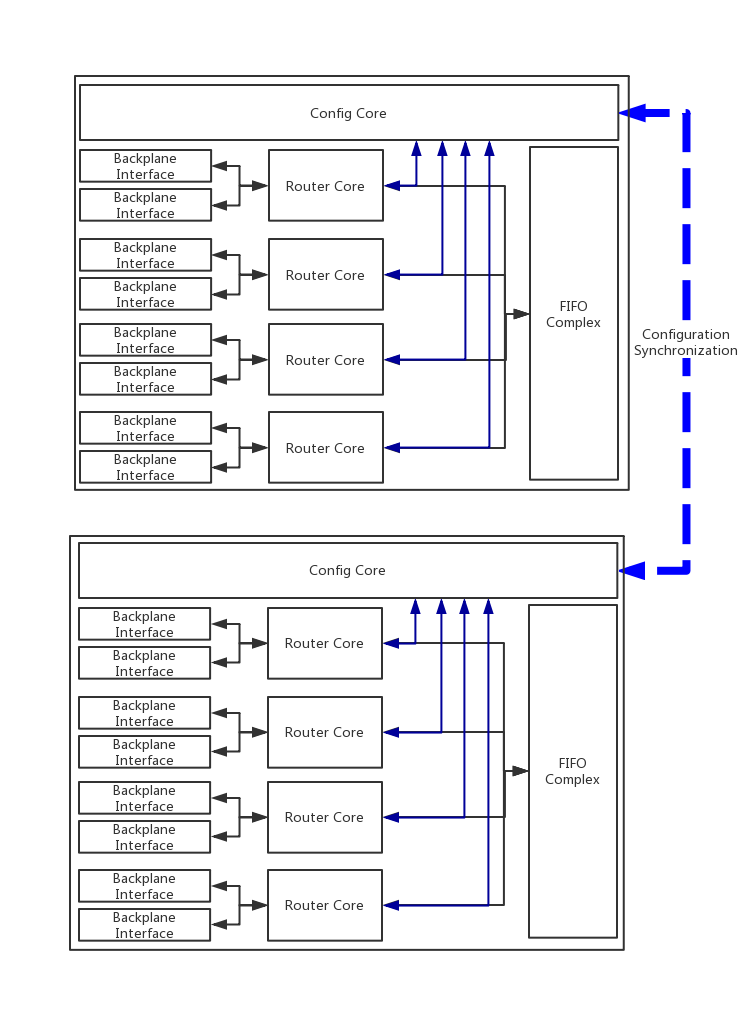
\includegraphics[width=0.7\textwidth]{img/DR00001_SpaceWire_2.png}
 \caption{Data Router Structure}
\end{center}
\end{figure}
\clearpage
\section{CAN + SpaceWire}
\subparagraph{Command Bus}CAN
\subparagraph{Data Bus}SpaceWire\\\\
In this plan, the command bus is using CAN. It provide prioritized data transmission for small amounts of data transmission, up to 500kbps bandwidth, which is enough bandwidth for command data transmission. The data bus is using SpaceWire which provides enough bandwidth for this high speed data transmission. It also includes a timestamp feature that will help in future sensor fusion. The whole system is build based on two routers, one is the main router that will be used for the major data transmission and the other is a backup router which can take over in the event the main router fails.
\begin{figure}[htp]
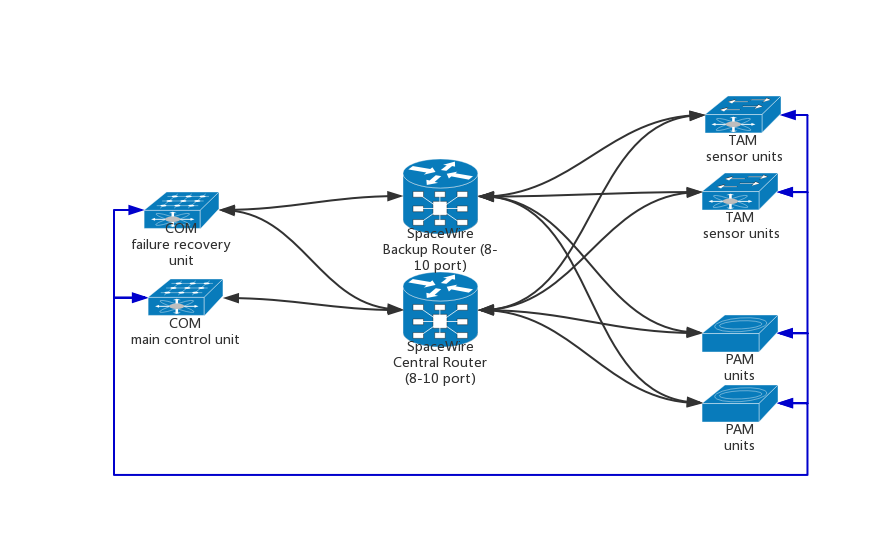
\includegraphics[width=\textwidth]{img/DR00001_SpaceWire_1.png}
 \caption{Recommand Design A}	
\end{figure}
\clearpage
\section{CAN + RapidIO}
\subparagraph{Command Bus}CAN
\subparagraph{Data Bus}RapidIO\\\\
In this plan, CAN bus still is the main command bus due to its prioritized data transmission. In the data bus, RapidIO each lane can carry 10 times data rate compared to SpaceWire. It can handle most future advanced missions without any hardware upgrades. A company will also be providing ASIC for rapidIO bus router.
\begin{figure}[htp]
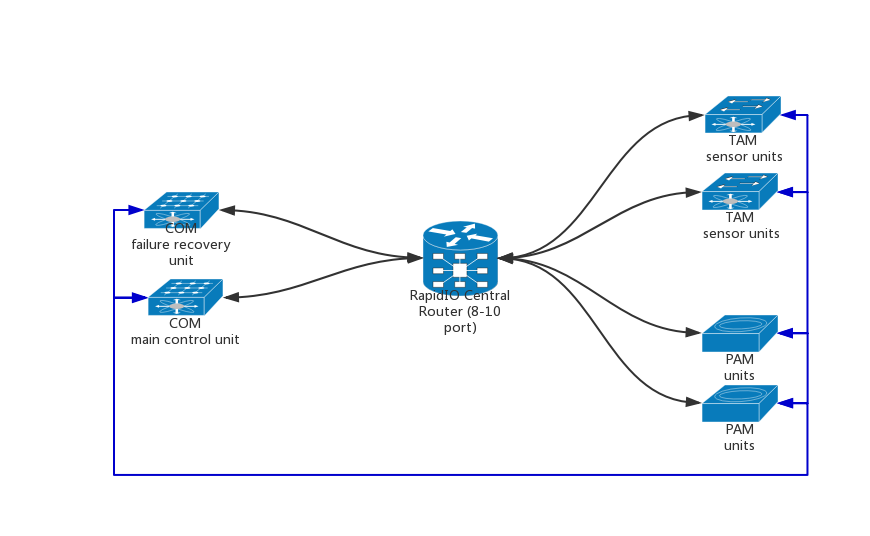
\includegraphics[width=\textwidth]{img/DR00001_RapidIO.png}
 \caption{Recommand Design B}	
\end{figure}
\newpage
%\chapter{OA-II BUS Software Structure}
%\newpage
%end of document
%**********************************************************************
\end{document}
